\section{Introduction}
\label{sec:intro}

The revolution in next-generation nucleotide sequencing has provided profound insights into the genetic composition and variation within biological samples and has yielded a number of scientific breakthroughs including <<pick your favorite examples>>. This scientific work has been supported by investments in fundamental research, technology and infrastructure and the resultant decrease in nucleotide sequencing and data storage costs have led to an exponential increase in the volume of sequence data generated by the scientific community. 
%<<Include some examples of exciting scientific work that relies on sequence data here to draw folks in>>

\subsection{The NIH Sequence Read Archive has reached the petabyte scale}
\label{sec:SraGrowth}

The Sequence Read Archive (SRA) at the National Institutes of Health is a diverse collection of next generation nucleotide sequencing data hosted by the National Center for Biotechnology (NCBI) at the National Library of Medicine (1,2). SRA provides a repository where data creators can share their raw sequence data with the scientific community and holds both public data available to all researchers and controlled access data derived from human research studies for use by qualified biomedical investigators who agree in advance to use the data appropriately. Sequence data in the archive is linked to associated metadata that provides information about the sequenced sample and can be used to associate genetic information in SRA with phenotypic, clinical, and environmental attributes [cite] \cite{katz2021stat}. The archive is also part of the International Nucleotide Sequence Database Collaboration (INSDC), and SRA sequence data and associated metadata as well as analogous data submitted to the European Nucleotide Archive (ENA) are exchanged among member databases.

\begin{figure}[t]
        \centering
        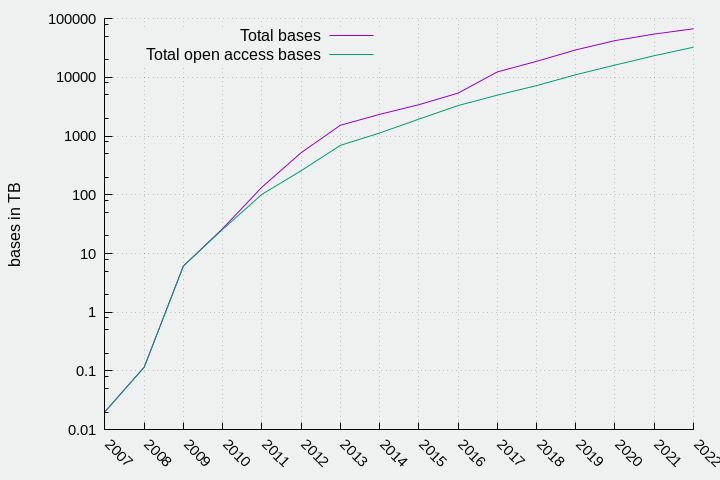
\includegraphics[width=0.6\textwidth]{images/sra_bases_TB.png}
        \caption{Growth of SRA. Databases like the NIH Sequence Read Archive are growing rapidly and are used extensively by scientific communities. As these databases grow, so do their potential scientific value, but work must be done to ensure ease of access.}
        \label{fig:sragrowth}
\end{figure}

The growth in nucleotide sequencing data within the scientific community has led to an explosion in the size of SRA (as seen in Figure 1 \ref{fig:sragrowth}), 
%Do we additional updates to Figure 1??
and there are now more than 16.8 million submitted samples from across all the domains of life that together comprise more than 17 petabytes of raw sequencing data in the repository (1,2). Given its vast size and diversity, the SRA represents a crucial resource for the scientific community, and researchers have developed bioinformatic tools and methods and tools that support deep analysis of SRA data – everything from assembly and annotation of genomes, characterization of human pathogens, discovery of novel organisms and viruses, and association of genetic signatures from complex microbiome and metagenomic samples with environmental attributes, to prediction of the functional significance of rare human genetic variation [cites].

To sustain future growth and facilitate expanded use the petabyte-scale SRA dataset, NIH partnered with Google Cloud Platform (GCP) \cite{GCP} and Amazon Web Services (AWS) \cite{AWS} in 2019, through the NIH Science and Technology Research Infrastructure for Discovery, Experimentation, and Sustainability (STRIDES) Initiative \cite{stridesini}. This partnership was part of a larger NIH STRIDES effort to build a cloud-enabled biomedical dataverse, with new processes, tools, and architecture to drive development of an equitable ecosystem that makes NIH-funded data findable, accessible, interoperable, and reusable (FAIR) \cite{wilkinson2016fair}. The entirety of the SRA sequence dataset is now replicated on Google and Amazon cloud platforms, and associated BioProject, BioSample, and SRA metadata is available through Google Big Query and Amazon Athena services. The public SRA dataset is available in normalized format through the AWS Open Data Program, and data can be egressed without charge into cloud and local locations \cite{sracosts}. 
%Is this a good place for talking about the cloud in terms of storage, access, and compute or should this go into a separate section?

\subsection{Petabyte-scale sequence search will improve the scientific impact of SRA}
\label{sec:psss}

While staging on cloud platforms provides enhanced access to SRA, successful use of the archive will require the basic ability to search across the petabyte-scale dataset to locate samples of interest. Search in this context can be thought of as two discrete functions: (1) text-based search, where queries to are matched to metadata descriptors associated with deposited sequence samples, and (2) sequence-based search, where sequence strings are matched to the sequence content of a sample. Attribute-based search depends on accurate sample metadata and is hindered by missing, incorrect, or inconsistently labeled or formatted metadata [3 plus other cites]. In contrast, sequence-based search is essentially agnostic to the sample information provided by data submitters and depends instead on the content of the sequence data itself.

Sequence-based search was critical to the application of GenBank as a public genetic sequence repository. The Basic Local Alignment Search Tool (BLAST) provided a way for researchers to compare experimentally derived sequences to those in the GenBank and to identify sequences of interest, such as [~2 EXAMPLES] [cites]. BLAST now supports sequence-based searches using nucleotide and protein sequences, translated sequences, and sequence models.These different search modalities support the identification of sequences with extensive homology to the query as well as the identification of more divergent sequences.  Similar search functionality will be critical to the usability of SRA On one hand, the immense scale of the database (? times the size of GenBank) imposes unique challenges to sequence search tools. On the other hand, the same scale will provide unique scientific rewards if such tools are successfully implemented.

\subsubsection{The value of sequence-based search }
\label{sec:SeqSearch}

Recent work by the Serratus group demonstrates the potential of SRA-wide sequence search to identify novel viruses \cite{edgar2022petabase}. However,no extant tool supports easy search across , one size fits all approach to sequence based search, and search strategies vary with the specific use case and underlying data. In some cases exact nucleotide matches are desired, so that samples that include specific query sequences can be identified. In other cases, similar matches to the query are desired, like when searching for samples that include homologous genes or related organisms. These different use cases often require different technical solutions, and in the case of BLAST, different databases and algorithms are constructed to support explicit and domain based nucleotide and amino acid sequence searches [cite]. Therefore it is likely that different scientific domains will require different computational tools capable of searching SRA at the petabyte scale.

% Should there be another subsection here on "Recent studies using the Serratus"??

\subsubsection{Metadata Challenges }
\label{sec:MetadataChallenges}

When the scientist’s goal is discovery of what relevant data might be available in the repository, a direct search on sequence data circumvents issues with missing or inaccurate metadata. Improving the accuracy of metadata is challenging and is an active area of research and is outside the scope of this investigation. Tools such as Metaseek aggregate the SRA metadata and preliminary investigation shows that many SRA entries are incomplete. We are interested in the types of discovery that are possible if scientists can quickly determine all the datasets that contain a particular gene or genome. The metadata associated with those datasets may be inaccurate and that will decrease the utility in reusing that data. Current advances in the area of large language models may yield improvements in language alignment that make metadata-based search strategy more powerful by improving current and future metadata quality. 

\begin{figure}%
    \centering
    \subfloat[\centering Percent public SRA accessions by organism]{{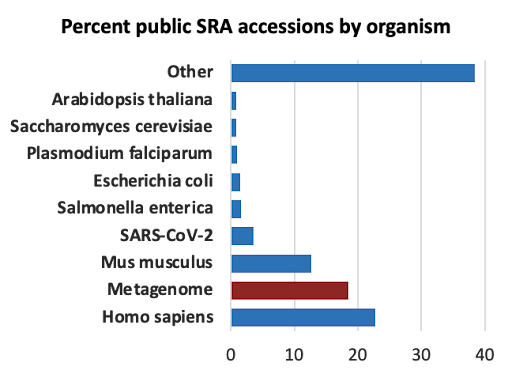
\includegraphics[width=7cm]{images/SRA_acc_organism.png} }}%
    \qquad
    \subfloat[\centering Percent public SRA accessions downloaded]{{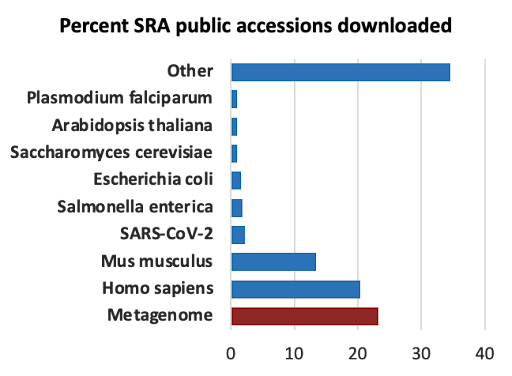
\includegraphics[width=7cm]{images/SRA_public_acc_downloaded.png} }}%
    \caption{SRA metagenomic accessions and usage}%
    \label{fig:metagenomicsradata}%
\end{figure}

\subsection{Metagenomics}
\label{sec:MetagenomicsData}

A metagenome is a dataset that represents a collection of genomes found in a sample. The sample may be from the human gut, a marine estuary, exotic locations, or your office. The study of the microbial communities is important because many phenomena are driven not just by the actions of a single microbial species, but many working together. Metagenomes are large, complex, and challenging to analyze, the largest dataset sizes are on the O(10TB). The field has benefited from a reduction in sequencing costs, as well as, more sophisticated data processing and analysis techniques that has led to an increase in the number of metagenomic studies. The number and size of metagenomic datasets being deposited and utilized in SRA is growing at a faster rate than other datasets.

\begin{itemize}
    \item SRA… and a large percentage of SRA data usage as seen in Figure \ref{fig:metagenomicsradata}
    \item Metagenomic datasets provide a unique set of challenges that include both known and unknown organisms within a sample
    \item Ability to identify organismal content and/or correlate it with sample attributes critical to use of metagenomic sequence datasets

\end{itemize}

\subsubsection{Examples of scientific inquiries/discoveries based on metagenomic analysis}
\label{sec:ExamplesOfMetadatAnalysis}

Challenge: as datasets get larger, and with long-read seq data, get more complete discrete genomes out. Especially w/ highly complex env samples. Can you leverage across existing sequence space to simplify the problem.



